\documentclass[crop,tikz]{standalone}
\usetikzlibrary{positioning,arrows,fit,calc}
\pgfdeclarelayer{bg}
\pgfsetlayers{bg,main}
\tikzset{
	>=stealth'
}
\begin{document}
	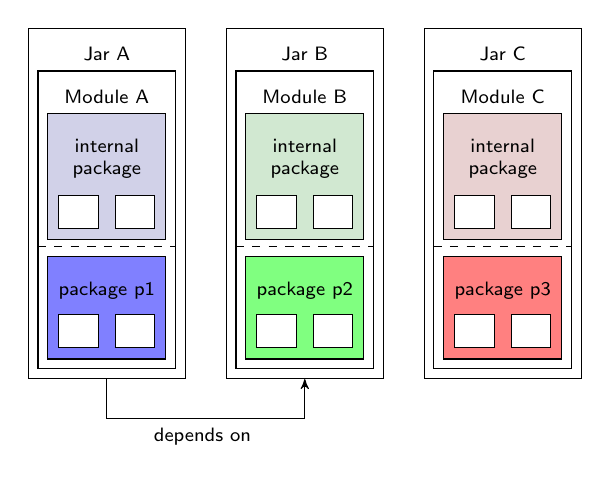
\begin{tikzpicture}[
	node distance = 2mm,
	every node/.style = {
		font = \sffamily\scriptsize
	},
	jar/.style = {
		draw,
		minimum height = 2.cm
	},
	package/.style = {
		draw,
		minimum height = 1.3cm,
		minimum width = 1.5cm
	},
	class/.style = {
		draw,
		fill = white,
		minimum height = \baselineskip,
		minimum width = .5cm
	}
	]
	
	\node (package_A1) [package, fill=blue!50] {};
	\node [below = of package_A1.north] {package p1};
	\node (class_1) [class, above right = of package_A1.south west] {};
	\node (class_2) [class, right = of class_1] {};
	
	\node (package_A2) [package, fill={rgb:blue,1;lightgray,4;white,6}, above = of package_A1, minimum height = 1.6cm] {};
	\node [below = of package_A2.north, text width=1.5cm, align = center] {internal package};
	\node (class_3) [class, above right = of package_A2.south west] {};
	\node (class_4) [class, right = of class_3] {};
	
	\node[fit=(package_A1)] (helpA) {};
	\draw[dashed] (helpA.north west) -- (helpA.north east);
	\node[above = 0mm of package_A2] (modA_title) {Module A};
	\node[draw, fit=(package_A1)(package_A2)(modA_title)] (modA) {};
	\node[above=0mm of modA] (jarAtitle) {Jar A};
	\node[draw, fit=(modA)(jarAtitle)] (jarA) {};
	
	
	\node (packageB1) [package, fill=green!50, right=1cm of package_A1] {};
	\node [below = of packageB1.north] {package p2};
	\node (class_5) [class, above right = of packageB1.south west] {};
	\node (class_6) [class, right = of class_5] {};
	
	\node (packageB2) [package, fill={rgb:green,1;lightgray,4;white,6}, above = of packageB1, minimum height = 1.6cm] {};
	\node [below = of packageB2.north, text width=1.5cm, align = center] {internal package};
	\node (class_7) [class, above right = of packageB2.south west] {};
	\node (class_8) [class, right = of class_7] {};
	
	\node[fit=(packageB1)] (helpB) {};
	\draw[dashed] (helpB.north west) -- (helpB.north east);
	\node[above = 0mm of packageB2] (modBtitle) {Module B};
	\node[draw, fit=(packageB1)(packageB2)(modBtitle)] (modB) {};
	\node[above=0mm of modB] (jarBtitle) {Jar B};
	\node[draw, fit=(modB)(jarBtitle)] (jarB) {};
	
	
	\node (packageC1) [package, fill=red!50, right=1cm of packageB1] {};
	\node [below = of packageC1.north] {package p3};
	\node (class_9) [class, above right = of packageC1.south west] {};
	\node (class_10) [class, right = of class_9] {};
	
	\node (packageC2) [package, fill={rgb:red,1;lightgray,4;white,6}, above = of packageC1, minimum height = 1.6cm] {};
	\node [below = of packageC2.north, text width=1.5cm, align = center] {internal package};
	\node (class_11) [class, above right = of packageC2.south west] {};
	\node (class_12) [class, right = of class_11] {};
	
	\node[fit=(packageC1)] (helpC) {};
	\draw[dashed] (helpC.north west) -- (helpC.north east);
	\node[above = 0mm of packageC2] (modCtitle) {Module C};
	\node[draw, fit=(packageC1)(packageC2)(modCtitle)] (modC) {};
	\node[above=0mm of modC] (jarCtitle) {Jar C};
	\node[draw, fit=(modC)(jarCtitle)] (jarC) {};
	
	\draw[->] (jarA.south) -- +(0,-0.5) -| node[below,xshift=-1.3cm] {depends on} (jarB);
		
	\end{tikzpicture}
	
\end{document}